\documentclass{rbfin}
\usepackage{amsmath}
\usepackage{amssymb} %mathbb
\usepackage{gensymb} % \degree
\usepackage{graphicx}
\usepackage{hyperref}
\usepackage{cancel}
\newcolumntype{C}{>{$}c<{$}}


\begin{document}
\selectlanguage{brazil}
\shorttitle{Identificação de Sistemas e Estimação de Parâmetros 2022} % appears on header every other page
\rbfe{}
\autor{Vinícius Claudino Ferraz, 2022}


\large

\begin{center}
LISTA 1
\end{center}

\normalsize

\doublespacing

\section*{Questão 1}

a) Simulado via MatLab.

b) Gráfico:

\begin{center}
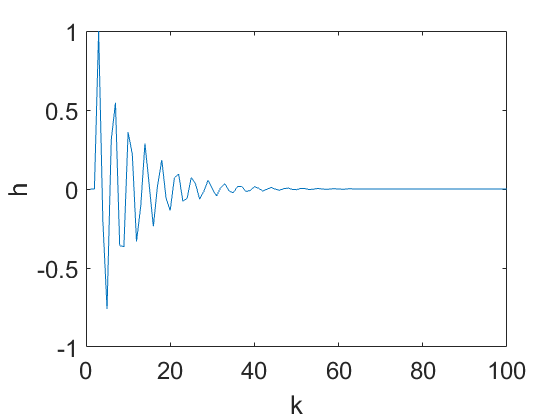
\includegraphics[scale=0.666]{q1}
\end{center}

c) A função de transferência é a razão entre a saída e a entrada: $H(z) = \cfrac{Y(z)}{U(z)}$ .

Multiplicando em cruz: $z^2 Y(z) + 0.2 z Y(z) + 0.8 Y(z) = U(z)$.

Queremos expoentes não positivos: $Y(z) + 0.2 z^{-1} Y(z) + 0.8 z^{-2} Y(z) = z^{-2} U(z)$.

Se $H(z) = \cfrac{N(z)}{D(z)}$, polinômio sobre polinômio, então multiplicamos por $z^{-d}$, em que $d = \deg D(z)$.

Pela transformada $\mathcal{Z}$ inversa: $y(k) + 0.2 y(k - 1) + 0.8 y(k - 2) = u(k - 2)$. 

Portanto, o atraso puro de tempo na entrada é igual a $2$. Isso aconteceu porque o grau do denominador é $2$ e o menor expoente do numerador é $0$. Se fosse $N(z) = a_1 z + a_2 z^2$, teríamos que subtrair $1$.

No caso geral, precisaríamos transformar $N(z) z^{-d}$ e o atraso puro de tempo seria $-(n - d) = d - n$, em que $n$ é o menor expoente do polinômio $N(z)$ de coeficiente não nulo.

\section*{Questão 2}

a) Simulado via MatLab. Eu queria forçar que $y(1) = 0.6$ e $y(2) = 0.5$. Para isso, considerei o vídeo no YouTube de título ``Observabilidade (ELT013)''. Utilizei a representação em espaço de estados. Inverti a matriz de observabilidade. E multipliquei pelo vetor de duas linhas conforme linha a seguir:

\footnotesize

\begin{verbatim}
x0 = obs * [y(1) - sys.D * u(1) ; y(2) - sys.C * sys.B * u(1) - sys.D * u(2)];
\end{verbatim}

\normalsize

b) Gráficos:

\begin{center}
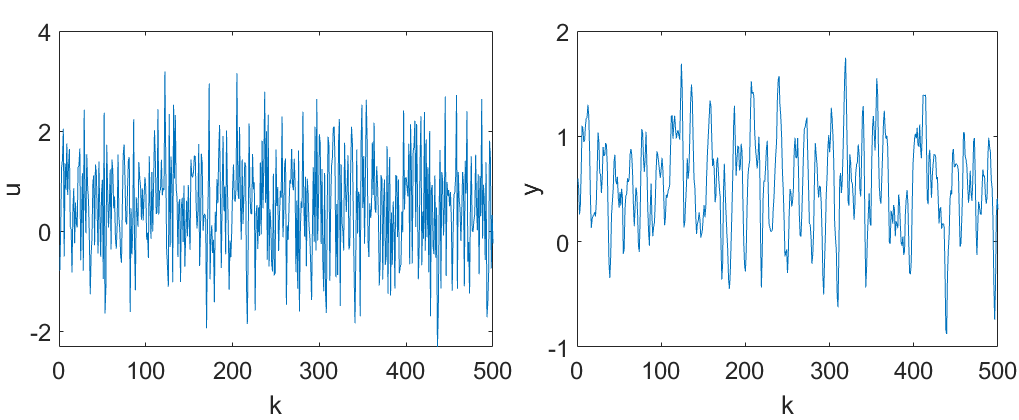
\includegraphics[scale=0.65]{q2}
\end{center}

c) Sim, a saída oscila um pouco menos que a entrada. Porque os sistemas físicos são passa-baixas.

\section*{Questão 3}

Salvei a entrada anterior em ``u.csv'' e recarreguei-a algumas vezes.

Mantive a saída do item $(2) = y$ e chamei a saída do ARX de $z$. A diferença entre o atual e o anterior foi pouca:

\begin{center}
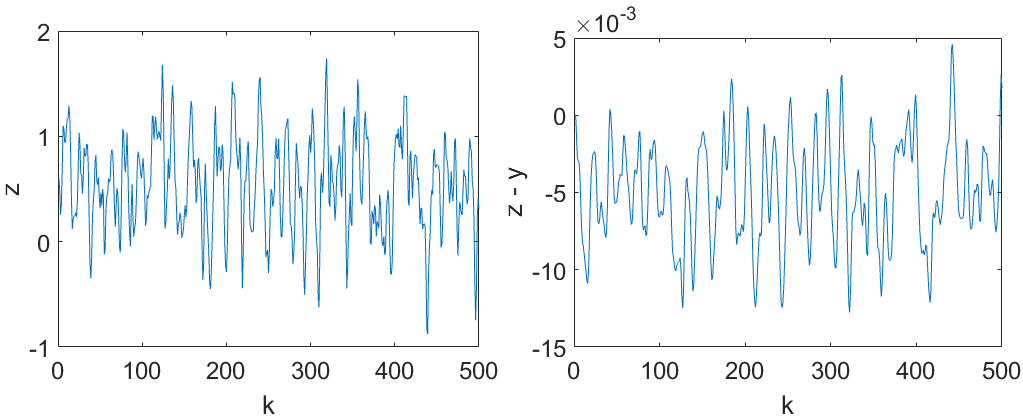
\includegraphics[scale=0.65]{q3z}
\end{center}

Com os $0.05 \sigma_z$ propostos, o ruído e a saída, denotada por $w$, foram:

\begin{center}
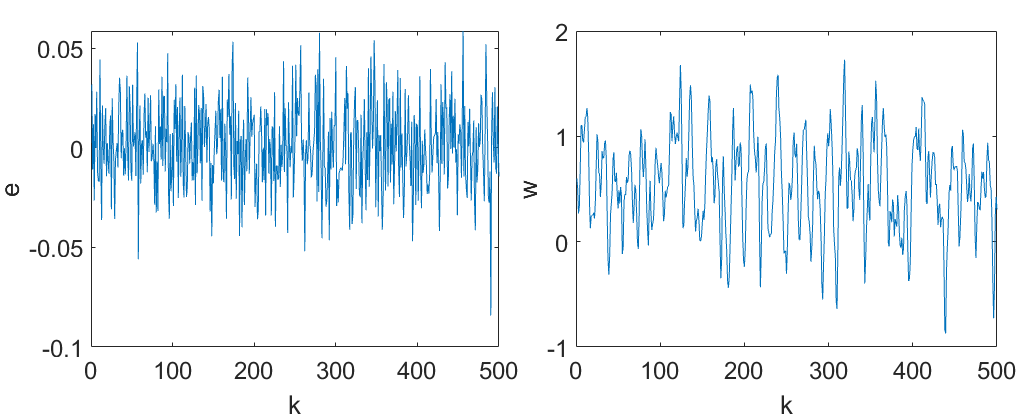
\includegraphics[scale=0.65]{q3ew}
\end{center}

A diferença entre esta última e a saída do item $(2) = y$ foi:

\begin{center}
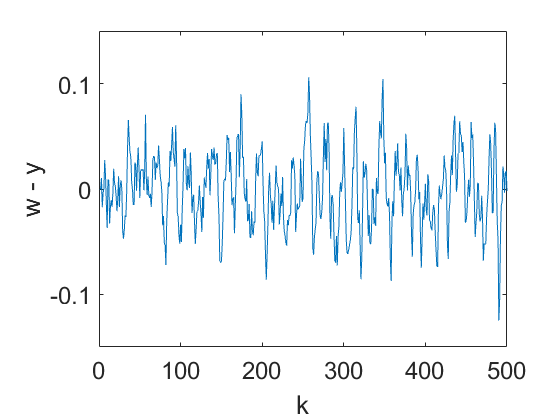
\includegraphics[scale=0.666]{q3wy}
\end{center}

\vspace{6mm}

Link para os \href{https://drive.google.com/file/d/1dgYeXCoKoHh6rJu9oeesB-6cMUV_UR9D/view?usp=sharing}{\color{blue}\underline{códigos-fonte}}.

Versão de 29/abril/2022\footnote{Fora da caridade não há salvação.} por Vinicius Claudino Ferraz. 

Matrícula: 2019435823.

\end{document}
